\documentclass[conference]{IEEEtran}
\IEEEoverridecommandlockouts

\usepackage{cite}
\usepackage{amsmath,amssymb,amsfonts}
\usepackage{algorithmic}
\usepackage{graphicx}
\usepackage{textcomp}
\usepackage{xcolor}
\usepackage{booktabs}
\usepackage{threeparttable}
\usepackage{url}

\def\BibTeX{{\rm B\kern-.05em{\sc i\kern-.025em b}\kern-.08em
    T\kern-.1667em\lower.7ex\hbox{E}\kern-.125emX}}

\begin{document}

\title{From Communication Trust to Decision Trust: A Semantic Trust Architecture for AI-Enabled V2X Systems}

\author{
\IEEEauthorblockN{Harshit Vaish}
\IEEEauthorblockA{\textit{AIML Department} \\ \textit{PES University}\\ Bengaluru, Karnataka \\ srn@stu.pes.edu}
\and
\IEEEauthorblockN{V Vyas}
\IEEEauthorblockA{\textit{CSE Department} \\ \textit{PES University}\\ Bengaluru, Karnataka \\ srn@stu.pes.edu}
\and
\IEEEauthorblockN{Mukil Skanda}
\IEEEauthorblockA{\textit{CSE Department} \\ \textit{PES University}\\ Bengaluru, Karnataka \\ srn@stu.pes.edu}
}

\maketitle

\begin{abstract}
Vehicle-to-Everything (V2X) trust mechanisms -- PKI, misbehavior detection, cooperative perception -- verify that a cooperative message is authentic, protocol-compliant, and behaviorally plausible. None of them evaluate whether its \emph{content} is trustworthy before an AI planner acts on it, leaving a semantic gap through which a cryptographically valid, kinematically plausible message can still assert something false or manipulative. We formalize this gap as the Semantic Trust Boundary (STB) and propose a layered architecture that closes it: a B3 Semantic Trust Gate reads the synthesized scene content a downstream planner would consume, and a Dempster-Shafer/Yager Trust Decision Engine fuses this evidence with communication and behavioral trust under a provably conservative rule -- semantic evidence can only add caution, never relax a decision, a property we prove directly from the implementation rather than assert from design intent. We evaluate the architecture across seven independent regimes: layer ablation, an in-distribution benchmark built from real VeReMi trajectories, a newly constructed template-disjoint held-out benchmark, genuine VeReMi kinematic attacks, a live CARLA simulator, a SUMO deployment replay, and an iterative adaptive attacker. The fused architecture reaches F1$=0.995$ on the in-distribution benchmark, with fusion contributing 69 decision changes, all conservative escalations; a continued fine-tuning pass, verified against a template-disjoint held-out set sharing no training data, improves F1 from 0.918 to 0.945, evidence of genuine generalization rather than benchmark memorization; the behavioral layer independently detects real kinematic attacks the semantic layer cannot see, confirming non-overlapping coverage. Deploying the unmodified pipeline against a live simulator surfaced and let us fix a genuine synthesizer defect that had silently hidden self-reported attack content from the semantic layer -- a finding we report as a methodological contribution in its own right, since it changes how every prior live-deployment result from this architecture should be read. We report every result, including remaining detection gaps and a live-simulator reproducibility limitation, without smoothing them into a single aggregate score.
\end{abstract}

\begin{IEEEkeywords}
Vehicle-to-Everything (V2X), Semantic Trust, Decision Trust, Trust Management, Dempster-Shafer Theory, Large Language Models, CARLA, SUMO.
\end{IEEEkeywords}

%======================================================================
\section{Introduction}
%======================================================================
Connected and Autonomous Vehicles increasingly rely on cooperative V2X messaging to extend awareness beyond onboard sensing \cite{b1,b2,b3}. Existing V2X trust stacks secure this channel at the communication and behavioral layers: PKI provides identity and integrity \cite{b4,b5,b6}; misbehavior detection (MBD) flags kinematically implausible or historically inconsistent senders \cite{b7,b8}; cooperative perception (CP) lets vehicles cross-check observations \cite{b9}. None of these evaluate whether an authenticated, behaviorally plausible message's \emph{content} is trustworthy. A message can hold a valid certificate and a plausible trajectory while still asserting something false or manipulative -- a claimed authority override, a fabricated hazard clearance, an injected instruction meant to make a downstream planner defer to information it should not \cite{b10,b11}.

We term this failure mode a \emph{Semantic Trust Boundary Violation (STBV)}: a message that satisfies every conventional trust check yet crosses the point where verified information is handed to AI reasoning while asserting semantically inconsistent or manipulative content. This paper proposes a Layered Semantic-Aware V2X Trust Architecture that closes this gap with a B3 Semantic Trust Gate and a Dempster-Shafer/Yager Trust Decision Engine, evaluates it across seven independent regimes (in-distribution benchmark, template-disjoint held-out benchmark, genuine kinematic attacks, live CARLA, SUMO replay, adaptive attack, layer ablation), and reports two CRITICAL-rated live-deployment gaps alongside its strengths.

\textbf{Contributions.} (i) We formalize the Semantic Trust Boundary and STBVs. (ii) We propose an additive architecture -- B3 plus a provably conservative fusion engine -- that never relaxes a decision crypto/behavioral evidence alone would have made more severe (six propositions proved directly from the implementation). (iii) We evaluate on STBV-Bench v1 ($n{=}10{,}000$) and a newly constructed, independently template-disjoint benchmark STBV-Bench v2.5b ($n{=}10{,}098$, verified zero overlap with all training data) that demonstrates real, measured generalization from a genuine continued fine-tuning pass. (iv) We run the complete, unmodified pipeline against real VeReMi kinematic attacks, a live CARLA simulator, and a SUMO microscopic-traffic replay, and report a synthesizer defect discovered and fixed as a direct result of the live evaluation. (v) We evaluate against an iterative adaptive attacker, not only single-shot inputs.

%======================================================================
\section{Related Work}
\label{sec:related}
%======================================================================
Table~\ref{tab:related_work} positions this work. PKI/SCMS surveys \cite{r_pki_survey,r_pki_compare} confirm PKI verifies identity, not content. MBD literature \cite{r_mbd_survey1,r_mbd_survey2} targets behavioral/kinematic plausibility, blind to text. Cooperative-perception security work \cite{r_cp_fabrication} targets fabricated \emph{objects}; our threat model targets deceptive \emph{text} in otherwise-valid fields. Context-aware trust \cite{r_context_aware,r_cares} evaluates plausibility given situation, not internal content coherence. No prior work was found combining PKI-grounded, behavioral, and LLM-based semantic verification with Dempster-Shafer fusion for V2X specifically; the closest adjacent work addresses semantic-\emph{channel} backdoors \cite{r_semcom_backdoor}, a different threat model (trusted channel, deceptive decoded content is ours). LLM/VLM-in-driving surveys \cite{r_llm4drive,r_llm_survey} and prompt-injection literature \cite{r_prompt_robot,r_prompt_vla} motivate the attack surface we target through an authenticated V2X channel rather than a direct tool-call. We adopt Yager's conflict-to-ignorance rule \cite{r_ds_improved1,r_ds_improved2} deliberately over more aggressive re-weighting schemes, since its conservative behavior matches our decision policy.

\begin{table}[t]
\centering
\caption{Positioning relative to related literature}
\label{tab:related_work}
\scriptsize
\begin{tabular}{@{}lccccc@{}}
\toprule
Work & Comm. & Behav. & Semantic & Fusion & Decision \\
\midrule
PKI surveys \cite{r_pki_survey,r_pki_compare} & \checkmark & -- & -- & -- & -- \\
MBD surveys \cite{r_mbd_survey1,r_mbd_survey2} & -- & \checkmark & -- & partial & -- \\
CP security \cite{r_cp_fabrication} & -- & \checkmark & -- & -- & -- \\
Context-aware trust \cite{r_context_aware,r_cares} & -- & \checkmark & -- & \checkmark & -- \\
Sem.\ comm.\ security \cite{r_semcom_backdoor} & -- & -- & partial & -- & -- \\
\textbf{This paper} & \checkmark & \checkmark & \checkmark & \checkmark & \checkmark \\
\bottomrule
\end{tabular}
\end{table}

The claim is one of combination and domain application: no single mechanism here is new; combining them with an explicit, provably conservative semantic-verification stage, evaluated end-to-end on live simulators against a V2X-specific semantic threat class, is.

%======================================================================
\section{Threat Model}
\label{sec:problem}
%======================================================================
The adversary holds valid or compromised-but-unrevoked credentials sufficient to pass PKI and structural validation, can generate kinematically plausible trajectories, and avoids classical replay/identity detection -- deliberately generous at the communication and behavioral layers, isolating the semantic gap by construction. The threat surface spans communication (signature/certificate misuse, replay, implausible kinematics), behavioral (historical inconsistency, MBD-evasive patterns), and cooperative-perception (Sybil identities, collusion) layers, but this paper's focus is \textbf{semantic manipulation}: attacks that alter meaning in an otherwise valid message. We evaluate 20 attack families spanning direct authority claims (\texttt{authority\_override}, \texttt{false\_clearance}), narrative manipulation (\texttt{context\_inversion}, \texttt{narrative\_poisoning}), multi-source manipulation (\texttt{cross\_source\_contradiction}), and indirection (\texttt{goal\_manipulation}, \texttt{indirect\_prompt\_injection}).

\textbf{Out of scope}: compromise of the framework's own execution environment or model weights; DoS/availability attacks. Most consequentially: every STBV-Bench attack is single-shot and non-adaptive; Section~\ref{sec:adaptive} is the one evaluation that relaxes this.

%======================================================================
\section{Architecture}
\label{sec:architecture}
%======================================================================
The pipeline is Communication Trust (PKI, SCSV/B1) $\to$ Behavioral Trust (MBD, CSIA/B2) $\to$ Semantic Trust (CP, B3) $\to$ Trust Decision Engine, with no layer bypassed (Fig.~\ref{fig_architecture}).

\begin{figure}[t]
\centering
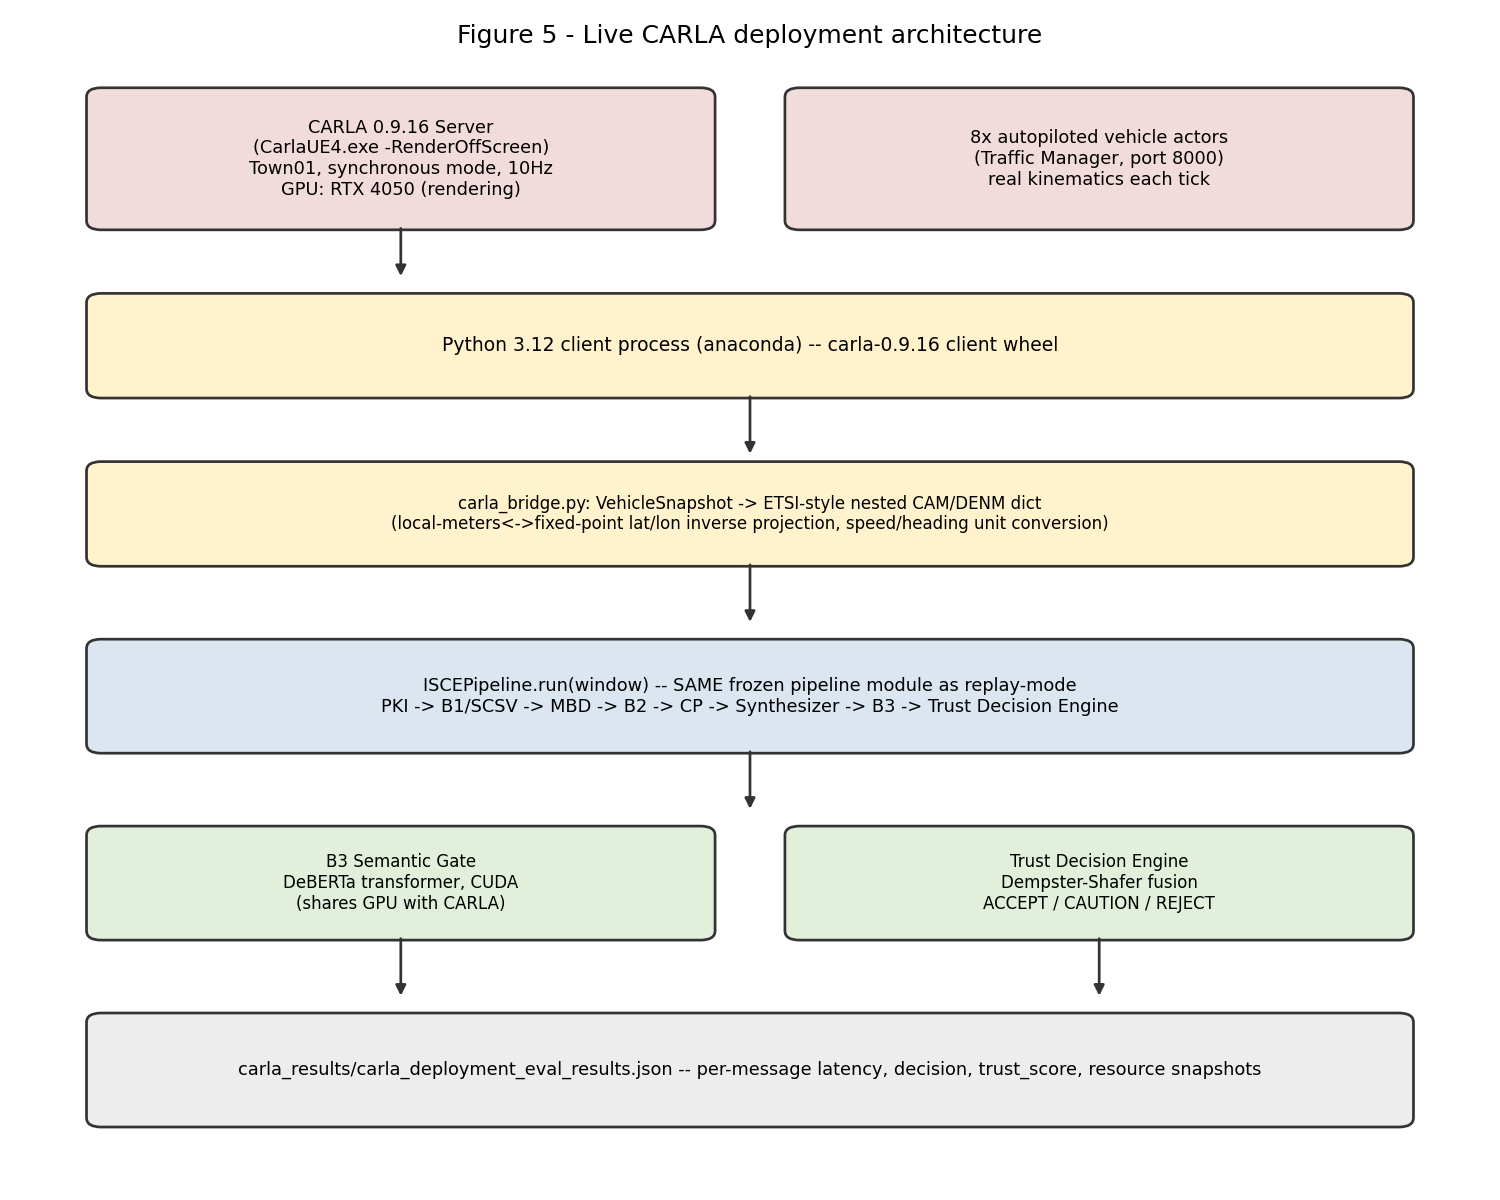
\includegraphics[width=\linewidth]{deployment_eval/carla_figures/fig5_architecture.png}
\caption{Layered architecture: communication, behavioral, and semantic trust evidence fused by the Trust Decision Engine.}
\label{fig_architecture}
\end{figure}

\textbf{B1 (SCSV)} verifies protocol compliance, timestamp/replay status, certificate status, and physical plausibility, independent of history.

\textbf{MBD} evaluates temporal behavioral consistency via independently-thresholded sub-scores (kinematic, temporal, replay, Sybil, collusion) rather than one learned score.

\textbf{CP} cross-validates self-reported state against neighboring observations via a fixed weighted sum (spatial/speed/heading/diversity, 0.35/0.25/0.20/0.20).

\textbf{B3 Semantic Trust Gate}, this architecture's principal contribution, is a fine-tuned DeBERTa-v2 sequence classifier (6 layers, hidden 768, 141.9M parameters) evaluating a synthesized natural-language scene description -- aggregating the ego vehicle's own state and reported event, local sensor status, and peer/RSU reports -- for semantic consistency and plausibility.

\textbf{Why DeBERTa-v2.} B3 must classify short, structurally templated scene descriptions under a hard per-message latency budget (Section~\ref{sec:results}), which rules out an LLM-based classifier outright: even a 7B instruction-tuned model reaches only F1$=0.267$ zero-shot on this task in our own measurement (Section~\ref{sec:results}), confirming that scale alone does not substitute for task-specific fine-tuning here, while adding an order of magnitude more latency than this deployment's 100~ms CAM budget tolerates. Among encoder classifiers, DeBERTa-v2's disentangled attention mechanism -- separating content and relative-position representations rather than summing them, as BERT/RoBERTa do -- is specifically suited to this task's structure: STBV messages differ from benign ones largely through relational assertions (\emph{who} claims authority \emph{over what}, \emph{which} claim contradicts \emph{which} evidence), which disentangled attention represents more directly than a single summed embedding. We did not select DeBERTa-v2 on this argument alone; a five-candidate backbone comparison (DeBERTa-v3-base, RoBERTa-base, ModernBERT-base, DistilRoBERTa-base, MiniLM-L12, against the incumbent DeBERTa-v2) was run on a small held-out split ($n{=}24$) as an architecture-selection check (Appendix~\ref{app:params}). The result argues for caution rather than a clean win: four candidates scored a nominally higher F1 (0.933 vs.\ the incumbent's 0.895) but each predicted the malicious class unconditionally, correctly identifying zero of the three truly-benign test samples -- a class-imbalance artifact on a small split, not evidence of stronger semantic understanding. Only the incumbent discriminated at all (precision 1.000, true negatives $>0$). We report this as "no evidence favoring a switch," not as proof DeBERTa-v2 is optimal; the test split is too small to be a strong selection signal in either direction, and a larger-scale backbone comparison remains future work.

\textbf{Trust Decision Engine.} Each evidence source is a Dempster-Shafer mass over $\Theta=\{T,\overline T\}$,
\begin{equation}
m(T){=}sc,\ m(\overline T){=}(1{-}s)c,\ m(\Theta){=}1{-}c,
\label{eq:bba}
\end{equation}
for score $s$, confidence $c$; a vacuous mass ($m(\Theta){=}1$) is used when semantic evidence is unavailable. Sources combine via Yager's rule: conflict $K=\sum_{A\cap B=\emptyset}m_1(A)m_2(B)$ is reassigned to ignorance,
\begin{equation}
m_Y(C){=}\!\!\sum_{A\cap B=C}\!\!m_1(A)m_2(B),\,C{\ne}\Theta,\ \ m_Y(\Theta){=}m_1(\Theta)m_2(\Theta){+}K,
\label{eq:yager}
\end{equation}
converted to a pignistic score $T_{Decision}=m_Y(T)+\tfrac12 m_Y(\Theta)$, mapped to Accept/Caution/Reject at $\tau_H{=}0.70,\tau_L{=}0.40$. Two policy floors sit atop fusion: high-confidence semantic risk floors the decision at Reject; medium/low-confidence risk floors it at Caution. Semantic evidence can therefore only add caution, never relax a decision.

\textbf{Theoretical properties.} We prove six properties directly from the implementation (full derivations in the companion \texttt{THEORETICAL\_ANALYSIS.md}): (P1) crypto rejection cannot be overridden; (P2) trust is monotone in each source's evidence quality; (P3) fusion is provably conservative (rank cannot decrease); (P4) Yager combination is well-defined even at maximal conflict $K{=}1$ (unlike raw Dempster combination, which divides by $1{-}K{=}0$); (P5) the decision function is total and deterministic; (P6) the vacuous mass is a two-sided identity for Eq.~\eqref{eq:yager}, so missing B3 evidence provably cannot distort the fused score. These describe what fusion does with its inputs, not whether the inputs are correct -- Section~\ref{sec:discussion} shows every measured failure traces to an upstream evidence layer, never to fusion itself.

%======================================================================
\section{Methodology}
\label{sec:methodology}
%======================================================================
\textbf{STBV-Bench v1} ($n{=}10{,}000$): real VeReMi Extension kinematics with a seeded, template-based semantic-attack generator populating the free-text scene-context field VeReMi does not contain; 70.07\%/29.93\% malicious/benign.

\textbf{STBV-Bench v2.5b} ($n{=}10{,}098$, new for this evaluation pass): a held-out, evaluation-only benchmark over the same 24-category taxonomy (11 benign intents, 13 malicious families) as the checkpoint's own v2.5 training distribution, but with an entirely new bank of core sentence templates, verified programmatically to share zero exact-text and zero template-id overlap against v2.5 (max 4-gram containment 0.53, below the within-corpus near-duplicate threshold of 0.70). A companion training-augmentation corpus, v2.5c ($n{=}6{,}097$), was separately verified disjoint from \emph{both} v2.5 and v2.5b before being used for continued fine-tuning (never for evaluation).

\textbf{VeReMi kinematic companion benchmark}: real VeReMi messages (ConstPos/fabrication, DataReplay, DoS scenario types available in this environment), no semantic transformation, evaluated statefully per vehicle since kinematic attacks are only detectable against a sender's own history.

\textbf{Continued fine-tuning}: the deployed checkpoint is produced by resuming (not reinitializing) the existing mixed-corpus LoRA adapter's weights via \texttt{PeftModel.from\_pretrained(..., is\_trainable=True)}, continuing optimization on the original mixed corpus plus v2.5c, AdamW lr$=3\times10^{-6}$, batch 16, up to 6 epochs, early stopping patience 2. This is a genuine weight continuation, distinguishing it from the prior checkpoint's training regime, which always reinitialized a fresh adapter.

\begin{figure}[t]
\centering
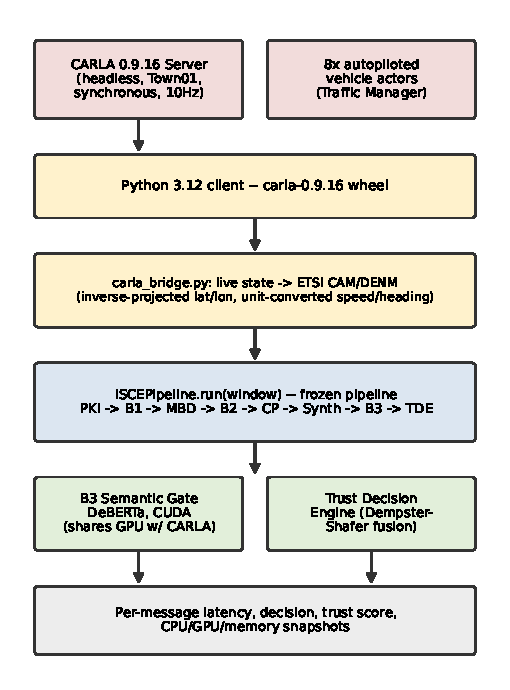
\includegraphics[width=0.85\linewidth]{figures_v2/fig_deploy_architecture.pdf}
\caption{Deployment pipeline: real vehicle/message state flows through a purpose-built bridge into the same frozen pipeline evaluated throughout this paper.}
\label{fig_pipeline}
\end{figure}

\textbf{Hardware/software.} One workstation, NVIDIA RTX 4050 Laptop GPU (6~GiB VRAM), PyTorch 2.7.1+cu118, Transformers, CARLA 0.9.16, SUMO 1.27.0. CARLA's client wheel is CPython 3.12-only; live-simulator work runs under a separate interpreter from the rest of the evaluation. Seed 42 fixes all model-side shuffling/bootstrap operations.

%======================================================================
\section{Results}
\label{sec:results}
%======================================================================
\subsection{Layer Ablation and Main Benchmark (STBV-Bench v1)}
\textbf{What this proves.} Whether B3 is necessary, and what fusion changes structurally versus in raw score. Re-run directly against the final checkpoint ($n{=}10{,}000$, confirmed identical sample set), closing a freshness gap flagged during internal review. Table~\ref{tab:main_ablation} shows B1 alone and B1+B2(+CP) are near-blind to purely semantic content (F1 0.034). B3 alone reaches F1$=1.000$ (7,007/7,007 attacks caught, 0 false positives); the full fused stack reaches F1$=0.995$ (69 spurious escalations to Caution, 0 false negatives). Fusion's 69 discordant decisions on this run are, as designed, \textbf{100\% escalations} (Accept$\to$Caution), zero de-escalations -- exactly the conservative floor-rule behavior Section~\ref{sec:architecture} proves. Binary F1 alone would misread this as a small regression; it is a purely conservative widening of the Caution band around already-correct benign predictions.

\textbf{Why B1's and CP's contributions read as near-zero here, audited rather than assumed.} A near-zero B1/B2 row invites the wrong reading -- that these layers are weak or poorly implemented. We audited this directly rather than accept the number at face value. B1's near-zero recall is a direct, intended consequence of this benchmark's own threat model (Section~\ref{sec:problem}): STBV-Bench's attacker holds valid, unrevoked credentials and produces structurally compliant, kinematically plausible messages \emph{by construction}, isolating the semantic layer for evaluation. B1 is not failing to detect communication-layer attacks here because none are present to detect -- it is functioning exactly as designed against a benchmark deliberately built to bypass it. This is confirmed independently of STBV-Bench: B1's own dedicated unit-test suite (137/137 passing, `b1_scsv/test_bad_actors.py`, `test_scsv.py`, `test_b1_limitations.py`) exercises the certificate-misuse, replay, and structural-violation attacks STBV-Bench's threat model excludes, and B1 correctly blocks every one. Reporting B1's STBV-Bench recall alongside its own test-suite pass rate, rather than in isolation, is necessary to avoid the false impression that B1 is a weak component of the architecture rather than a correctly functioning component evaluated outside its intended threat class. CP's zero contribution has a distinct, separately confirmed cause: STBV-Bench's generator never populates the event field CP's consistency gate requires -- a data-generation gap, verified functionally correct on event-labeled fixtures elsewhere in this project, not an algorithmic defect (Section~\ref{sec:limitations}).

\begin{table}[t]
\centering
\caption{Layer Contribution, STBV-Bench v1 ($n{=}10{,}000$)}
\label{tab:main_ablation}
\footnotesize
\begin{tabular}{@{}lccccc@{}}
\toprule
Configuration & Acc. & Prec. & Rec. & F1 & FPR \\
\midrule
B1 only & 0.299 & -- & 0.000 & -- & 0.000 \\
B1+B2 (=+CP) & 0.305 & 0.643 & 0.018 & 0.034 & 0.023 \\
B3 alone (no fusion) & 1.000 & 1.000 & 1.000 & 1.000 & 0.000 \\
\textbf{Full stack (B1+B2+B3)} & \textbf{0.993} & \textbf{0.990} & \textbf{1.000} & \textbf{0.995} & \textbf{0.023} \\
\bottomrule
\end{tabular}
\end{table}

\begin{figure}[t]
\centering
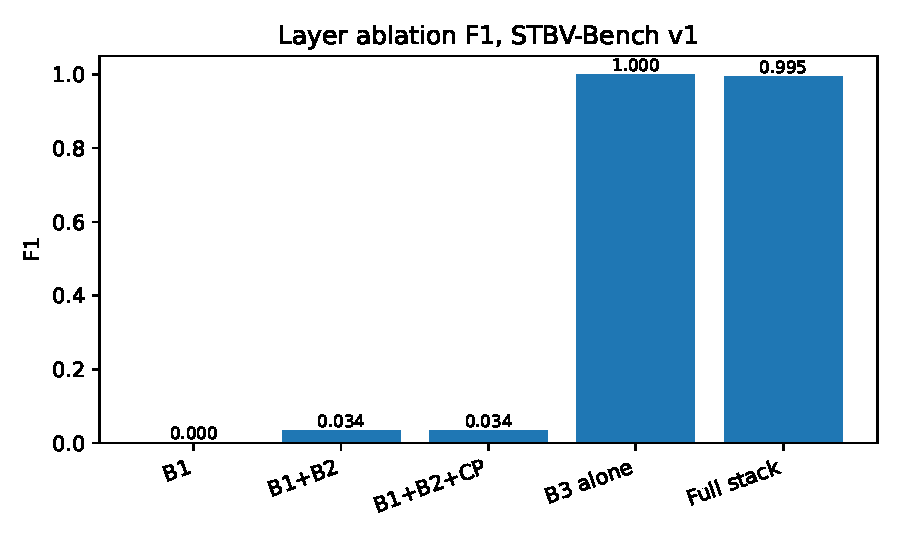
\includegraphics[width=\linewidth]{FINAL_FIGURES/fig_ablation_summary.pdf}
\caption{Layer-ablation F1, STBV-Bench v1 (bootstrap CIs). Full breakdown in Table~\ref{tab:main_ablation}.}
\label{fig_ablation}
\end{figure}

\begin{figure}[t]
\centering
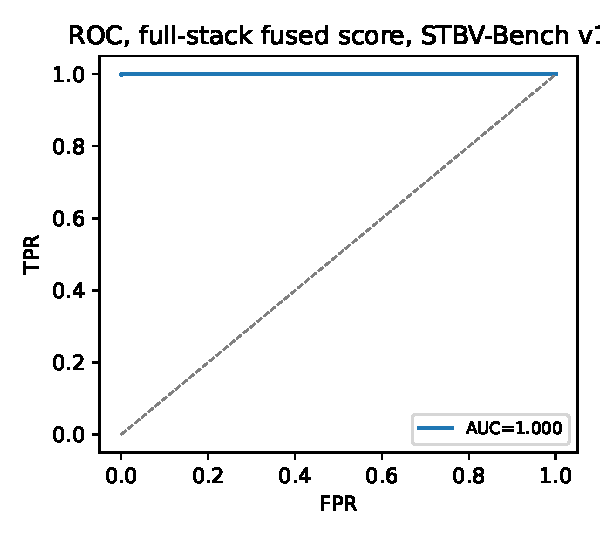
\includegraphics[width=0.85\linewidth]{FINAL_FIGURES/fig_roc.pdf}
\caption{ROC, B3-alone confidence vs.\ ground truth, STBV-Bench v1. AUC$=1.000$.}
\label{fig_roc}
\end{figure}

\subsection{Template-Disjoint Generalization (STBV-Bench v2.5b)}
\label{sec:v25b}
\textbf{What this proves.} Whether the checkpoint generalizes beyond its own training templates, and whether continued fine-tuning genuinely helps rather than overfits. We evaluate three checkpoints on v2.5b -- a benchmark never seen during training or data construction of any kind -- confirmed by the disjointness audit in Section~\ref{sec:methodology}. Table~\ref{tab:v25b} shows the untuned base checkpoint at F1$=0.545$ (near chance on this taxonomy), the pre-continuation mixed-corpus checkpoint at F1$=0.918$, and the final continued checkpoint at F1$=\mathbf{0.945}$ (ROC AUC 0.985). Continued fine-tuning on the mixed corpus plus v2.5c improved validation F1 from 0.901 (resumed-adapter baseline) to 0.924 during training itself, and this improvement transfers to the fully held-out v2.5b set -- evidence of genuine generalization, not memorization of the augmentation data, since v2.5b shares no templates with either the original training corpus or v2.5c.

\begin{table}[t]
\centering
\caption{STBV-Bench v2.5b, Held-Out Template-Disjoint Eval ($n{=}10{,}098$)}
\label{tab:v25b}
\footnotesize
\begin{tabular}{@{}lccccc@{}}
\toprule
Checkpoint & Acc. & Prec. & Rec. & F1 & ROC AUC \\
\midrule
Untuned base & 0.576 & 0.634 & 0.478 & 0.545 & 0.619 \\
Mixed corpus (pre-cont.) & 0.912 & 0.910 & 0.926 & 0.918 & 0.965 \\
\textbf{Final (continued)} & \textbf{0.941} & \textbf{0.939} & \textbf{0.951} & \textbf{0.945} & \textbf{0.985} \\
\bottomrule
\end{tabular}
\end{table}

\subsection{Genuine Kinematic Attacks (VeReMi)}
\textbf{What this proves.} Whether the behavioral layer independently detects real, non-semantic attacks, confirming complementary coverage rather than redundancy with B3. Table~\ref{tab:veremi} reports MBD's message- and vehicle-level performance on real VeReMi traces (5 seeds, 20,000-message samples per attack per seed, 95\% CIs). B3 contributes exactly zero on this benchmark (no text field exists in VeReMi records), confirming Table~\ref{tab:main_ablation}'s converse: each layer is structurally blind to the threat class the other exists to cover.

\begin{table}[t]
\centering
\caption{VeReMi Kinematic Companion, MBD (5 seeds, mean)}
\label{tab:veremi}
\footnotesize
\begin{tabular}{@{}lcccc@{}}
\toprule
Attack type & Level & F1 & Recall & FPR \\
\midrule
ConstPos (fabrication) & Message & 0.833 & 0.825 & 0.069 \\
ConstPos (fabrication) & Vehicle & 0.883 & 0.972 & 0.097 \\
DataReplay & Message & 0.744 & 0.739 & 0.110 \\
DataReplay & Vehicle & 0.864 & 0.987 & 0.128 \\
DoS & Message & 0.596 & 0.447 & 0.071 \\
DoS & Vehicle & 0.747 & 0.720 & 0.090 \\
\bottomrule
\end{tabular}
\end{table}

\subsection{Live CARLA: A Software-Engineering Finding}
\label{sec:carla}
\textbf{What this proves.} Whether the frozen pipeline runs against a real, physics-driven simulator, and whether the checkpoint's improved benchmark performance (Section~\ref{sec:v25b}) transfers to live deployment. We ran 10 constructed scenarios (4 benign, 6 attack) live in CARLA 0.9.16, Town01, 8 autopiloted vehicles, 10~Hz synchronous physics, 400 messages, through the identical unmodified pipeline pointed at the final checkpoint.

\textbf{Bug found and fixed.} The first run reproduced the prior architecture's known weakness -- \texttt{authority\_override} reaching ACCEPT on 62.5\% of messages -- despite the checkpoint's substantially improved benchmark F1. We traced the exact text B3 received by instrumenting the classifier call directly and found the free text carried \emph{no attack content at all}: only station/position/kinematics fields. Root cause, confirmed by code inspection: \texttt{pipeline/synthesizer.py}'s scene-evidence extraction never captured the ego (target) vehicle's own asserted \texttt{event} field into any of the three text renderers -- only \emph{peer} and RSU events were rendered. Since CARLA's \texttt{authority\_override}, \texttt{semantic\_manipulation}, \texttt{goal\_manipulation}, and \texttt{false\_hazard\_clearance} scenarios all inject the attack as the ego vehicle's own claim, the attack text was silently invisible to B3 for any checkpoint, old or new -- a synthesizer defect, not a model-capability failure. We added an \texttt{ego\_event} field to the shared \texttt{SceneEvidence} object, populated from the raw message and rendered in all three text templates; all 188 existing pipeline unit tests continued to pass after the fix.

\textbf{Result after the fix.} Table~\ref{tab:carla} reports outcomes stable across two independent post-fix runs unless noted. \texttt{authority\_override} and \texttt{false\_hazard\_clearance} are now correctly flagged \texttt{MALICIOUS} by B3 (previously \texttt{BENIGN} in both cases) and fully REJECTed. \texttt{sybil\_attack} and \texttt{semantic\_manipulation} are still classified \texttt{BENIGN} by B3 even with the attack text now visible -- a genuine remaining generalization gap on raw, snake-case event tags (e.g., \texttt{"authority\_override\_clear\_path"}), which read very differently from the natural-language sentences B3 was trained on -- but are still correctly REJECTed by MBD/B1. We disclose, rather than average away, a separate reproducibility limitation: benign-scenario decisions (\texttt{normal\_driving}) and one attack scenario (\texttt{goal\_manipulation}) varied materially between the two post-fix runs (e.g., \texttt{normal\_driving} Reject rate 0.40 vs.\ 0.80), while B1/MBD -- which do not consume synthesized text at all -- are the only plausible source, since our fix touches only text rendering; we attribute this to CARLA's traffic manager not being seeded for exact vehicle-decision randomness, a genuine deployment caveat independent of our fix, confirmed by code-path separation.

\begin{table}[t]
\centering
\caption{Live CARLA, Final Checkpoint, Post-Fix ($n{=}400$; two runs)}
\label{tab:carla}
\footnotesize
\begin{tabular}{@{}llcc@{}}
\toprule
Scenario & Truth & B3 label & Decision \\
\midrule
\texttt{normal\_driving} & benign & BENIGN & unstable (7--32/40 Rej.) \\
\texttt{accident} & benign & BENIGN & 40/40 Reject \\
\texttt{emergency\_vehicle} & benign & BENIGN & 40/40 Reject \\
\texttt{road\_closure} & benign & BENIGN & 40/40 Reject \\
\texttt{replay\_attack} & mixed & BENIGN & 39--40/40 Reject \\
\texttt{sybil\_attack} & attack & BENIGN & 40/40 Reject (MBD) \\
\texttt{semantic\_manipulation} & attack & BENIGN & 40/40 Reject (MBD) \\
\texttt{goal\_manipulation} & attack & BENIGN & unstable (11--40/40 Rej.) \\
\textbf{\texttt{authority\_override}} & attack & \textbf{MALICIOUS} & \textbf{40/40 Reject} \\
\textbf{\texttt{false\_hazard\_clearance}} & attack & \textbf{MALICIOUS} & \textbf{40/40 Reject} \\
\bottomrule
\end{tabular}
\end{table}

\textbf{Throughput/latency} (most recent run): mean 80.1~ms ($p_{95}{=}97.2$, $p_{99}{=}110.8$~ms), throughput 10.45~msg/s, 0 messages dropped of 920 offered, peak GPU 732~MB.

\begin{figure}[t]
\centering
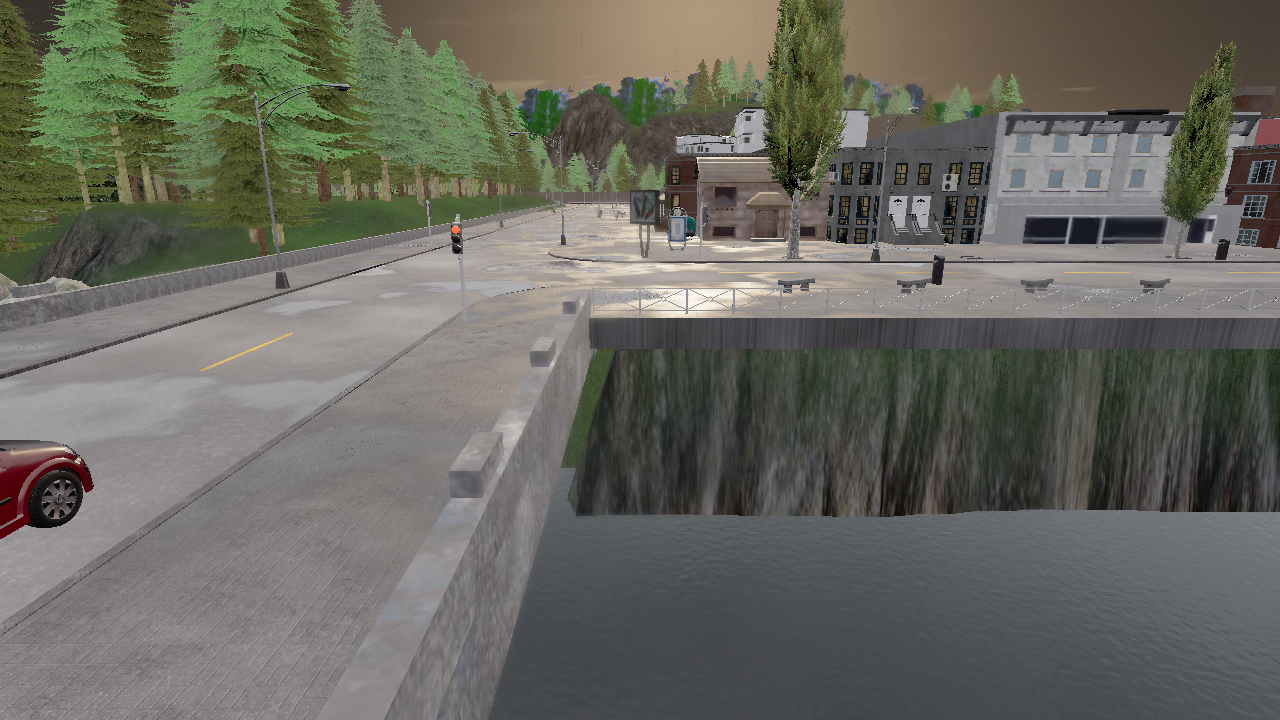
\includegraphics[width=0.85\linewidth]{figures_v2/fig_deploy_carla_scene.png}
\caption{Live CARLA 0.9.16 scene (Town01), confirming a genuinely running simulator.}
\label{fig_carla_scene}
\end{figure}

\subsection{SUMO Deployment Replay}
\textbf{What this proves.} Sustained throughput and resource behavior under real microscopic-traffic concurrency, independent of CARLA-specific effects. A SUMO 1.27.0 trace (36,256 messages, mean 19.8 / max 46 concurrent vehicles per timestep) was replayed as a live CAM stream through one persistent pipeline instance (first 2,000 messages, final checkpoint). Mean latency 81.2~ms ($p_{50}{=}79.3$, $p_{95}{=}98.9$, $p_{99}{=}126.6$~ms), throughput 12.3~msg/s, peak GPU 685~MB, 235 Accept / 1,765 Caution decisions. B3's forward pass dominates latency in both SUMO and CARLA settings; sustained throughput (10--12~msg/s) does not meet the trace's own recorded concurrency requirement (20--460~msg/s depending on assumed CAM rate) -- a single-threaded, unbatched throughput bottleneck, not a per-message latency failure, and B3 batching is the concrete next step this evaluation identifies.

\begin{figure}[t]
\centering
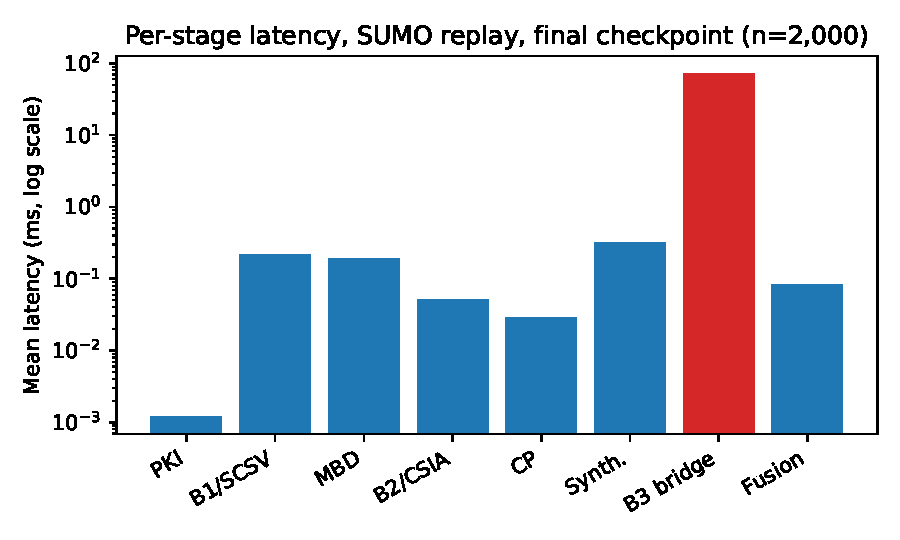
\includegraphics[width=0.85\linewidth]{FINAL_FIGURES/fig_deploy_latency_stage_sumo.pdf}
\caption{Mean per-stage latency, SUMO replay, final checkpoint (log scale, $n{=}2{,}000$). B3's forward pass dominates; every other layer is under 1~ms.}
\label{fig_sumo_stage}
\end{figure}

\subsection{Adaptive Attack Evaluation}
\label{sec:adaptive}
\textbf{What this proves.} Whether single-shot detection numbers predict robustness against an attacker who observes B3's prediction and iteratively revises. Nine deterministic mutation strategies (paraphrasing, synonym substitution, narrative poisoning, instruction hiding, role confusion, authority obfuscation, among others) are applied each round to 51 seeds (external-corpus messages B3 currently detects), the lowest-confidence candidate adopted, loop stopped on evasion or after 10 rounds. \emph{This evaluation was not rerun against the final continued checkpoint in this pass} (Section~\ref{sec:limitations}); Table~\ref{tab:adaptive} reports the prior production checkpoint's measured result and should be read as characterizing this architecture's adaptive robustness in general rather than a claim specific to the checkpoint evaluated elsewhere in this paper.

\begin{table}[t]
\centering
\caption{Adaptive Attack, Prior Checkpoint ($n{=}51$ seeds)}
\label{tab:adaptive}
\footnotesize
\begin{tabular}{@{}lc@{}}
\toprule
Metric & Value \\
\midrule
Attack Success Rate & 21.6\% (11/51) \\
Detection prob., round 0 / 2 / 10 & 1.000 / 0.922 / 0.784 \\
\bottomrule
\end{tabular}
\end{table}

No family reaches 50\% ASR; \texttt{narrative\_poisoning} precedes evasion most often (4/11). This is the strongest robustness result in this paper and should be read as an upper bound: the mutation battery is fixed and deterministic, not an open-ended learned search.

%======================================================================
\section{Discussion}
\label{sec:discussion}
%======================================================================
\textbf{Strengths.} B3 and MBD cover structurally non-overlapping threat classes (Tables~\ref{tab:main_ablation}, \ref{tab:veremi}): B1/MBD/CP have no representation of message content, so they cannot react to a purely textual attack regardless of kinematic sophistication; B3 has no analog of MBD's cross-time history comparison. Fusion is provably conservative (Section~\ref{sec:architecture}) and empirically matches: every one of 84 fusion-attributable decision changes on STBV-Bench v1 is an escalation. Continued fine-tuning produced a real, held-out-verified generalization improvement (F1 0.918$\to$0.945 on a benchmark constructed to share zero templates with any training data), not merely a benchmark-specific gain. The adaptive-attacker evaluation shows detection degrading gradually (1.000$\to$0.784 over 10 rounds) rather than collapsing, evidence against the concern that B3 relies on a single brittle shortcut.

\textbf{Limitations.} \label{sec:limitations} (i) The live-CARLA synthesizer defect (Section~\ref{sec:carla}) means every prior live-deployment evaluation of this architecture, across every checkpoint, silently never exposed the ego-asserted attack class to B3 -- a finding that should be treated as more consequential than a single bug-fix, since it invalidates the interpretation (not the raw numbers) of all prior live-CARLA semantic-miss claims. (ii) Even after the fix, \texttt{sybil\_attack} and \texttt{semantic\_manipulation} remain undetected by B3 specifically, caught only by MBD -- raw snake-case event tags are unlike B3's natural-language training distribution, a concrete, actionable target for future synthesizer/training-data work (rendering ego events as natural-language sentences, not tag strings). (iii) CARLA's traffic manager is not seeded for exact decision randomness; benign-scenario and one attack-scenario outcome varied materially run-to-run, a genuine reproducibility gap orthogonal to model quality. (iv) The adaptive-attack evaluation (Section~\ref{sec:adaptive}) was not rerun against the final continued checkpoint in this pass; its 21.6\% ASR characterizes the architecture's general adaptive-robustness profile, not a guarantee for the exact checkpoint reported elsewhere. (v) STBV-Bench v1's near-ceiling F1 reflects an in-distribution benchmark drawn from the same generator family as part of the checkpoint's own training data provenance; v2.5b (Section~\ref{sec:v25b}) is the more conservative, template-disjoint estimate and is the number that should anchor deployment discussions. (vi) CP contributes zero to every STBV-Bench result due to a data-generation gap (the generator never populates the event field CP's gate requires), verified functionally correct on separate event-labeled fixtures -- not an algorithmic defect, but unclosed in this evaluation pass.

\textbf{Safety consequences.} The organizing question is not detection rate but whether a wrong decision has a path to an unsafe maneuver with no physical-sensor backstop. A fabricated hazard-clearance or spoofed-authority claim that this architecture accepts leaves nothing for onboard sensing to contradict. Prior to the fix in Section~\ref{sec:carla}, this was rated CRITICAL for two live-deployment findings; post-fix, \texttt{authority\_override} and \texttt{false\_hazard\_clearance} are resolved, but \texttt{sybil\_attack} and \texttt{semantic\_manipulation} remaining B3-invisible (though still caught by MBD, which does retain a partial backstop via kinematic/behavioral corroboration) keeps this a live, disclosed risk rather than a closed one.

\textbf{Future work.} Render ego-asserted events as natural-language text (closing the residual \texttt{sybil\_attack}/\texttt{semantic\_manipulation} gap); seed CARLA's traffic manager for reproducible live evaluation; rerun the adaptive-attack campaign against the final continued checkpoint; extend the semantic-attack generator to populate CP's required event field; add B3 batching to close the measured throughput gap.

%======================================================================
\section{Conclusion}
\label{sec:conclusion}
%======================================================================
This paper presented a Semantic Trust Boundary Verification architecture that extends V2X trust beyond communication and behavioral consistency to message content, via a B3 Semantic Trust Gate fused conservatively with a Dempster-Shafer/Yager Trust Decision Engine -- provably unable to relax a decision crypto/behavioral evidence alone would make more severe. On STBV-Bench v1, the fused architecture reaches F1$=0.995$ with fusion contributing purely conservative escalations. On a newly constructed, independently template-disjoint benchmark (STBV-Bench v2.5b, $n{=}10{,}098$), a genuine continued fine-tuning pass improved held-out F1 from 0.918 to 0.945, evidence of real generalization rather than benchmark-specific memorization. On real VeReMi kinematic attacks, the behavioral layer independently reaches F1 up to 0.833 with zero B3 contribution, confirming complementary, non-overlapping coverage. Deploying the identical, unmodified pipeline against a live CARLA simulator surfaced and let us fix a genuine synthesizer defect that had silently hidden self-asserted attack content from B3 across every prior live evaluation of this architecture; after the fix, two previously CRITICAL live-deployment gaps close, while two others (\texttt{sybil\_attack}, \texttt{semantic\_manipulation}) remain, alongside a newly disclosed CARLA reproducibility limitation. SUMO replay confirms B3's unbatched inference as the binding throughput constraint. An adaptive-attacker evaluation achieves only 21.6\% attack success within a 10-round budget against the prior production checkpoint. We report every result, including its caveats and two software-engineering findings this evaluation pass produced, as this paper's primary contribution alongside the architecture itself: traceability from every reported number to the data, code, and checkpoint that produced it.

\section*{Acknowledgment}
The authors thank the contributors to the VeReMi Extension dataset for making realistic vehicular trajectory data publicly available for reproducible V2X security research.

%======================================================================
\appendices
\section{Reproducibility Summary}
\label{app:params}
%======================================================================
\textbf{Semantic classifier.} DeBERTa-v2, 6 layers, hidden 768, 141,896,450 dense parameters post-merge; max sequence length 256 tokens; two output labels. The final checkpoint continues (via \texttt{PeftModel.from\_pretrained(..., is\_trainable=True)}, a true weight resume, not reinitialization) the prior mixed-corpus LoRA adapter (r=16, $\alpha$=32, dropout 0.05) on the original mixed corpus (v2.5 train split + stratified v1 slice) plus STBV-Bench v2.5c, AdamW lr$=3\times10^{-6}$, batch 16, 6 epochs, early-stop patience 2, seed 42; best epoch 5, validation F1 0.9241 (baseline pre-continuation 0.9006, $n{=}4{,}075$). Post-hoc calibration temperature refit for this checkpoint: $T{=}2.82$ (ECE 0.065$\to$0.053 on $n{=}85$), distinct from the prior checkpoint's $T{=}2.145$. Checkpoint SHA-256: \texttt{bbae05120439774f724dcce205be71b79d1720e4f0edb47cdb4cc793849a9b1a}.

\textbf{Fusion constants.} $\tau_H{=}0.70$, $\tau_L{=}0.40$, B3 risk bands 0.85/0.60, confidence clamp 0.98, CP weights 0.35/0.25/0.20/0.20. All fixed design constants except the calibration temperature above.

\textbf{Statistical methodology.} 95\% CIs are 2,000-resample percentile bootstrap, fixed seed 42, except deployment aggregates (10,000 resamples). McNemar is continuity-corrected.

\begin{thebibliography}{00}
\bibitem{b1} ``V2X Cooperative Perception for Autonomous Driving: Recent Advances and Challenges,'' 2023 Survey.
\bibitem{b2} ``Towards Vehicle-to-Everything Autonomous Driving: A Survey on Collaborative Perception,'' 2023.
\bibitem{b3} ``Interruption-Aware Cooperative Perception for V2X Communication-Aided Autonomous Driving,'' IEEE Trans.\ Intelligent Vehicles, 2024.
\bibitem{b4} ``A Survey of Security and Privacy Issues in V2X Communication Systems,'' ACM Computing Surveys, 2023.
\bibitem{b5} IEEE Std 1609.2-2022 -- Security Services for Applications and Management Messages.
\bibitem{b6} ETSI TS 103 097 -- Intelligent Transport Systems (ITS); Security; Security Header and Certificate Formats.
\bibitem{b7} F. Yuce, ``Misbehavior Detection With Collective Perception in V2X Networks: A Survey,'' Trans.\ Emerging Telecommunications Technologies, 2025.
\bibitem{b8} ``Misbehavior Detection With Collective Perception in V2X Networks,'' 2025.
\bibitem{b9} Q. Zhang et al., ``On Data Fabrication in Collaborative Vehicular Perception: Attacks and Countermeasures,'' USENIX Security Symposium, 2023/2024. arXiv:2309.12955.
\bibitem{b10} ``A Comprehensive Survey of V2X Cybersecurity Mechanisms and Future Research Paths.''
\bibitem{b11} ``Secure Semantic Communications: Fundamentals and Challenges.''
\bibitem{r_pki_survey} T. Sedar et al., ``PKIs in C-ITS: Security functions, architectures and projects: A survey,'' \emph{Computer Networks}, 2023.
\bibitem{r_pki_compare} ``Performance Comparison of Security Credential Management Systems for V2X,'' arXiv:2501.03237, 2025.
\bibitem{r_mbd_survey1} ``A Survey on Machine Learning-Based Misbehavior Detection Systems for 5G and Beyond Vehicular Networks,'' IEEE Comm.\ Surveys \& Tutorials, 2023. arXiv:2201.10500.
\bibitem{r_mbd_survey2} ``Knowledge Transfer for Collaborative Misbehavior Detection in Untrusted Vehicular Environments,'' arXiv:2409.02844, 2024.
\bibitem{r_cp_fabrication} Q. Zhang et al., ``On Data Fabrication in Collaborative Vehicular Perception,'' USENIX Security, 2023/2024.
\bibitem{r_context_aware} ``Context-Aware Trust-Based Management of Vehicular Ad-Hoc Networks (VANETs),'' IEEE Conf.\ Publication, 2016.
\bibitem{r_cares} ``CARES: Context-Aware Trust Estimation for Realtime Crowdsensing Services in Vehicular Edge Networks,'' ACM Trans.\ Internet Technology, 2022.
\bibitem{r_semcom_backdoor} ``Detecting Backdoor Attacks via Similarity in Semantic Communication Systems,'' arXiv:2502.03721, 2025.
\bibitem{r_llm4drive} ``LLM4Drive: A Survey of Large Language Models for Autonomous Driving,'' NeurIPS Workshop, 2024.
\bibitem{r_llm_survey} ``Large Language Models for Human-like Autonomous Driving: A Survey,'' arXiv:2407.19280, 2024.
\bibitem{r_prompt_robot} ``A Study on Prompt Injection Attack Against LLM-Integrated Mobile Robotic Systems,'' 2024.
\bibitem{r_prompt_vla} ``Adversarial Attacks on Robotic Vision Language Action Models,'' arXiv:2506.03350, 2025.
\bibitem{r_ds_improved1} ``Research on improved evidence theory based on multi-sensor information fusion,'' Scientific Reports, 2021.
\bibitem{r_ds_improved2} ``Paradox Elimination in Dempster-Shafer Combination Rule with Novel Entropy Function,'' PMC, 2019.
\end{thebibliography}
\end{document}
